\documentclass[hidelinks,12pt,a4paper]{article}
\usepackage{rotating}
\usepackage[utf8]{inputenc}
\usepackage[T1]{fontenc}
\usepackage[ngerman]{babel}
\usepackage{here}
\usepackage{listings} 
\lstset{language=XML} 
\usepackage{xcolor}
\usepackage{tikz}
\usepackage{tabularx}
\usepackage{booktabs, multicol, multirow}
\usepackage{rotating}
\usepackage{bigstrut}
\usepackage{svg}
\usepackage{wrapfig}
\usepackage{pdfpages} 
\usepackage{floatflt}
\usepackage{amsmath, amssymb}
\usepackage[printonlyused]{acronym} 
\usepackage{textcomp}
\usepackage{url}
\usepackage{caption}
\usepackage[export]{adjustbox}
\def\UrlBreaks{\do\/\do-}

\clubpenalty10000
\widowpenalty10000
\displaywidowpenalty=10000


\lstdefinelanguage{JavaScript}{
	keywords={typeof, new, true, false, catch, function, return, null, catch, switch, var, if, in, while, do, else, case, break},
	keywordstyle=\color{blue}\bfseries,
	ndkeywords={class, export, boolean, throw, implements, import, this},
	ndkeywordstyle=\color{darkgray}\bfseries,
	identifierstyle=\color{black},
	sensitive=false,
	comment=[l]{//},
	morecomment=[s]{/*}{*/},
	commentstyle=\color{purple}\ttfamily,
	stringstyle=\color{red}\ttfamily,
	morestring=[b]',
	morestring=[b]",
	extendedchars=true,
	basicstyle=\footnotesize\ttfamily,
	showstringspaces=false,
	showspaces=false,
	numberstyle=\footnotesize,
	numbersep=9pt,
	numbers=left,
	tabsize=2,
	breaklines=true,
	showtabs=false,
	captionpos=b,
	xleftmargin=20pt
}

\lstset{literate=%
	{Ö}{{\"O}}1
	{Ä}{{\"A}}1
	{Ü}{{\"U}}1
	{ß}{{\"ss}}1
	{ü}{{\"u}}1
	{ä}{{\"a}}1
	{ö}{{\"o}}1
	{~}{{\textasciitilde}}1
}

%\usepackage{hyperref}
\usetikzlibrary{arrows,shapes,snakes,automata,backgrounds,petri}
\lstdefinestyle{base}{
	language=xml,
	emptylines=1,
	breaklines=true,
	basicstyle=\ttfamily\color{black},
	moredelim=**[is][\color{red}]{@}{@},
}


\newcommand{\autorPraxisbericht}{Florian Zoia}
\newcommand{\titelPraxisbericht}{Marketing Automation für Inbound Sales Strategien und der Auswahl einer entsprechenden Software}
\newcommand{\titelVeranstaltung}{{\sl Praxisbericht}}
\newcommand{\ersterBetreuer}{Prof. Dr. Peter Manshausen}
\newcommand{\fach}{Betriebswirtschaftslehrer II}
\newcommand{\abgabeortPraxisbericht}{Frankfurt am Main}
\newcommand{\datumAbgabePraxisbericht}{\today}



\usepackage[ngerman]{babel}
\usepackage{times}
\usepackage{natbib}
\usepackage{pdfpages}
\usepackage{amssymb}
\usepackage{amsmath}
\usepackage{graphicx}
\usepackage{svg}
\usepackage{eurosym}
\usepackage{txfonts}
\usepackage{pifont}
\usepackage{url}
\usepackage{colortbl}
\urlstyle{tt}
\usepackage{tikz}
\usepackage{pgflibrarysnakes}
\usetikzlibrary{shadows,fadings}
\usetikzlibrary{decorations}
\usetikzlibrary{arrows} % LATEX and plain TEX when using Tik Z


%\usepackage[paper=a4paper, 
%%outer=15mm, 
%%inner=30mm, 
%%top=40mm, 
%%bottom=25mm, 
%bindingoffset=10mm]{geometry} 



\definecolor{white}{gray}{1.00}
\definecolor{black}{gray}{0.00}
\definecolor{skyblue}{cmyk}{0.4, 0.2, 0.0, 0.0}             % HKS44-40
\definecolor{blue}{cmyk}{1.0, 0.5, 0.0, 0.0}                % HKS44-100
\definecolor{lightblue}{cmyk}{0.7, 0.35, 0.0, 0.0}          % HKS44-70
\definecolor{darkblue}{rgb}{0.04, 0.16, 0.32}               % 
\definecolor{extradarkblue}{cmyk}{1.00, 0.70, 0.10, 0.50}   % HKS41-100
\definecolor{darkgreen}{cmyk}{1.0, 0.0, 0.9, 0.2}           % HKS57-100
\definecolor{green}{cmyk}{0.65, 0.0, 1.0, 0.0}              % HKS65-100
\definecolor{purple}{cmyk}{0.5, 1.0, 0.0, 0.0}              % HKS33-100
\definecolor{indigo}{cmyk}{0.8, 0.9, 0.0, 0.0}              % HKS36-100
\definecolor{gray}{gray}{0.59}
\definecolor{lightgray}{gray}{0.4}
\definecolor{darkgray}{gray}{0.50}
\definecolor{darkcyan}{cmyk}{0.87, 0.4, 0.4, 0.0}
\definecolor{cyan}{cmyk}{0.78, 0.19, 0.01, 0.0}
\definecolor{lightcyan}{cmyk}{0.39, 0.095, 0.005, 0.0}
\definecolor{extralightcyan}{cmyk}{0.16, 0.1, 0.0, 0.0}
\definecolor{beetleBlue}{RGB}{64,80,127}

\usepackage[
colorlinks=false,
urlcolor=black,
linkcolor=black
]{hyperref}

\setlength{\textwidth}{15.5cm}     %
\setlength{\textheight}{23cm}      %
\setlength{\evensidemargin}{0cm} %
\setlength{\oddsidemargin}{0.95cm}  %
\setlength{\topmargin}{-1cm}       %
\setlength{\topskip}{0cm}          %
\setlength{\headheight}{11pt}      %



%\setlength{\textwidth}{15.5cm}     %
%\setlength{\textheight}{23cm}      %
%\setlength{\evensidemargin}{1.5cm} %
%\setlength{\oddsidemargin}{1.5cm}  %
%\setlength{\topmargin}{-1cm}       %
%\setlength{\topskip}{0cm}          %
%\setlength{\headheight}{11pt}      %


\title{%
	\titelPraxisbericht\\%
	\vspace{8mm}{\large Praxisbericht im Studiengang}\\%
	{\LARGE Bachelor Business Information Management}\\%
	{\large an der}\\%
	{\LARGE Provadis - School of International}\\%
	{\LARGE Management and Technology}\\%
}

\author{%
	{\normalsize vorgelegt von}\\%
	\vspace{4mm}\autorPraxisbericht\\%
	{\normalsize im Fach}\\
	{\LARGE \fach}\\
	\vspace{4mm}~\\{\normalsize Betreuer}\\%
	\ersterBetreuer}

\date{
	\vfill\abgabeortPraxisbericht, \datumAbgabePraxisbericht\\%
	~\\%
	
\includegraphics[scale=.75]{ComLogo.png}\hfil
	
\includegraphics[scale=.22]{ProvadisLogo.png}%
}


\newcommand{\Lab}[3] { %
 \put(#1,#2){\makebox(0,0){\shortstack[c]{#3}}}%
}

\newcommand{\lb}{\linebreak}%
\newcounter{wMinipage}%
\newcommand{\tiktxt}[4]{%
\setcounter{wMinipage}{#3*\real{1.3}}
\draw(#1 mm,#2 mm) node {\begin{minipage}{\thewMinipage mm}\begin{center}\setlength{\baselineskip}{2.5ex} #4\end{center}\end{minipage}};%
}%
\newcommand{\rtiktxt}[5]{%
\setcounter{wMinipage}{#3*\real{1.3}}
\draw(#1 mm,#2 mm) node[rotate=#5] {\begin{minipage}{\thewMinipage mm}\begin{center}\setlength{\baselineskip}{2.5ex} #4\end{center}\end{minipage}};%
}%





\newcommand{\spw}{\glqq StaffIT pro\grqq{}}
\begin{document}
	
	\maketitle
	\thispagestyle{empty}
	
	\newpage
	\pagestyle{headings}
	
	
	\input{./Abschnitte/Erklärungen.tex}
	\newpage
	\pagestyle{headings}
	
	\newpage
	
	\pagestyle{headings}
	\section*{}
	\tableofcontents
	\newpage
	\addcontentsline{toc}{section}{Abbildungsverzeichnis}
	\listoffigures
	
	
	
	
	\newpage
	\pagenumbering{arabic}
	\setcounter{page}{1}
	
	\section{Einführung in das Thema}
	Diese Arbeit behandelt das Thema 'Lead Generierung für Inbound Sales Marketing'. Dabei wird erörtert, wie die Mail Adressen und weitere, für das Marketing Team, nützliche Daten gesammelt und weiterverarbeitet werden können. Diese Daten sollen für das Inbound Marketing in der COM-Software GmbH genutzt werden.
	
	\subsection{Einordnung in das Thema}
	Inbound Marketing spielt in der heutigen Welt eine große Rolle. Kunden wollen als Individuen gesehen werden und sprechen viel positiver auf personalisierte Werbung an. Dieses Konzept möchte sich die COM-Software GmbH ebenfalls zu Nutze machen und Werbungen schalten, bei denen die Kunden auf die COM-Software GmbH zukommen. Hierbei ist es notwendig bestimmte Kundendaten zu sammeln, um den Kunden immer wieder zu erkennen und spezifisch auf ihn Werbung schalten zu können.
	\newline
	Dafür wird in dieser Arbeit ermittelt, welche die besten Möglichkeiten sind, um an genau die notwendigen Daten zu kommen, um dem Kunden personalisiert Werbung zu schalten. 

	\subsection{Leitfrage}
	Wie kann die COM-Software GmbH Kundeninformationen sammeln und diese weiterverarbeiten, um damit Leads zu generieren und Neukundenakquise zu betreiben.
	
	\subsection{Ziel der Arbeit}
	Diese Arbeit beschäftigt sich mit der Gewinnung von Kundendaten und deren Weiterverarbeitung, um diese im Inbound Marketing zu nutzen. Hierbei werden die unterschiedlichen Methoden zum Erhalt und der Weiterverarbeitung von Kundendaten vorgestellt und erörtert, um den idealen Weg zu finden diese Informationen im Inbound Marketing der COM-Software GmbH nutzen zu können.
	
	\subsection{Aufbau der Arbeit}
	Anfangs wird diese Arbeit die Grundlagen aufführen, welche benötigt werden, um die Arbeit zu verstehen. Dazu zählen die Themen 'Inbound Marketing', 'Outbound Marketing', 'Marketing Automatisation' und 'Webscraping'.
	\newline
	Darauf folgen die verschiedenen Arten der Datenbeschaffung und wie man diese weiterverarbeiten kann, um den Kunden damit werben zu können. Anschließend werden diese Möglichkeiten gegenübergestellt, um deren Vor- und Nachteile zu erarbeiten und die beste Möglichkeit für die COM-Software GmbH zu finden.
	\newline
	Im Fazit wird ermittelt, welche dieser Möglichkeiten am besten geeignet ist, um in der COM-Software GmbH umgesetzt werden zu können.
	
	\subsection{Forschungsmethode}
	Die Grundlagen der Arbeit wurden durch eine Literaturrecherche mit Hilfe der angegebenen Fachliteratur und einer Internetrecherche erarbeitet.
	
	
	
	
	
	\newpage
	\section{Grundlagen zur Bearbeitung}
Für das Projektverständnis sind Grundlagen zu schaffen. Sowohl die Einordnung des Projektthemas
als auch die unterschiedlichen Tools, Informationssysteme und genutzten Methoden müssen verständlich erläutert sein, um den Gesamtkontext der Arbeit einordnen zu können.

\subsection{Inbound Marketing}
Inbound Marketing ist eine Art des Marketings, die auf personalisierter Werbung besteht und den Kunden zum Unternehmen bringen soll. Der Kunde soll, der Firma gegenüber, loyal und freundlich gesinnt sein. Dies wird durch personalisierte Werbung erreicht, bei welcher der Kunde nicht direkt vom Marketing Team angesprochen wird. Dafür werden Kundendaten benötigt, mit welchen die Firma gezielt Werbung schalten kann. Diese Werbung wird nicht nur auf der eigenen Plattform betrieben, sondern erreicht den Kunden über mehrere Kanäle. Somit bleibt das Unternehmen dem Kunden im Hinterkopf und wenn sich ein Problem entwickelt, bei welchem das Unternehmen eine Lösung anbietet wird sich der Kunde an das  Unternehmen wenden.
\newline 
Allerdings spielt nicht nur Werbung eine große Rolle im Inbound Marketing, da die potenziellen Kunden erst einmal auf das Unternehmen aufmerksam werden müssen. Dies geschieht durch gute Erfahrungen von Bekannten oder Kollegen, genauso wie die Vorstellung der eigenen Leistungen. Dies kann durch die eigene Website sein, Soziale Medien oder Blogs, welche vom Marketing Team gepflegt werden. Wird der potenzielle Kunde durch solche Informationen auf das Unternehmen aufmerksam, kann sich, über Cookies oder ähnliches, das Unternehmen den User merken und ihm gezielt Werbung schalten. Somit bleibt das Unternehmen im Gedächtnis des potenziellen Kunden und sobald dieser eine Leistung benötigt, welche das besagte Unternehmen anbietet, wird er an dieses denken und sich an das Unternehmen wenden. Genauso ist es wichtig bei Suchmaschinen wie 'Google', 'Bing' etc. weit oben zu sein. Dadurch kann der potenzielle Neukunde das Unternehmen schneller entdecken. Des Weiteren besuchen die wenigsten Menschen die zweite oder dritte Seite einer Suchmaschine, weshalb es sehr von Vorteil für ein Unternehmen ist, bei Suchmaschinen weit oben gelistet zu sein.
\newline 
Ein weiterer Teil des Inbound Marketings ist es nicht alle Informationen auf einmal Preis zu geben. Besucht ein potenzieller Kunde eine Website, so kann er meist alle Informationen einsehen. Beim Inbound Marketing wird dem potenziellen Kunden nur ein Bruchteil der möglichen Informationen geliefert. Um an weitere zu kommen ist es notwendig eine Mail Adresse oder andere Daten, welche das Unternehmen weiter für Werbung nutzen kann, zu hinterlegen. Somit kann sich der Kunde weiter informieren und zeigt sein ehrliches Interesse an dem Unternehmen und das Unternehmen erhält nötige Daten, welche für weitere Inbound Marketing Strategien genutzt werden kann. 
\newline 
Damit die Werbung richtig personalisiert werden kann ist es wichtig für das Unternehmen, dass es seine Zielkunden kennt. Hierfür werden 'Buyers Personas' und 'Ideal Customer Profile' angelegt. 
\newline 
Um ein 'Ideal Customer Profil' anzulegen, muss ein Unternehmen wissen, wie die eigenen Kunden ausschauen. Sind es andere Unternehmen, so sollte klar sein, wie viele Angestellte die Kunden im Durchschnitt haben, welches Budget ihnen zur Verfügung steht, wo die Sitze des Unternehmens liegen und wie lange die Projekte oder einzelnen Geschäftsbeziehungen im durchschnitt dauern. Mit Hilfe dieses 'Ideal Customer Profil' können Unternehmen ermitteln, ob ein potenzieller Kunde in das Schema des Unternehmens passt oder ob es die eigene Kapazität übersteigt. Außerdem kann mit dem 'Ideal Customer Profil' ermittelt werden, auf welchen Plattformen die Kunden am besten zu erreichen sind, da große Unternehmen anders operieren, als Mittelständige oder Kleinunternehmen. 
\newline 
Bei den 'Buyers Personas' wird geschaut, wer dafür Zuständig ist die Geschäfte mit der eigenen Firma abzuwickeln. Dabei wird festgestellt, ob es ein Abteilungsleiter oder CEO des Unternehmens ist. Des weiteren wird geschaut, worauf die einzelnen Kunden achten. Dabei werden die bestehenden Kunden analysiert, um festzustellen, wo Gemeinsamkeiten bestehen und inwiefern sich die einzelnen Kunden unterscheiden. Anhand dieser Informationen wird festgestellt, welche Herausforderungen die einzelnen Kunden mit sich bringen und wie diese spezifisch in der Werbung angesprochen werden können, um das eigene Angebot attraktiv zu machen. 
\newline 
Mit Hilfe der Buyers Personas' und 'Ideal Customer Profile', kann das Unternehmen beginnen die eigenen Kunden in Gruppen zu unterteilen. Zu diesen Gruppen werden die potenziellen Neukunden ebenfalls zugewiesen, um die Werbung so individuell und attraktiv wie möglich zu gestalten. Somit kann viel mehr auf die eigenen Interessen der verschiedenen Kunden und Neukunden eingegangen werden. Die bestehenden Kunden haben das Gefühl, dass das Unternehmen genau weiß, was die Kunden brauchen und die möglichen Neukunden zeigen schneller Interesse, da gleich auf die eigenen Probleme und Bedürfnisse eingegangen wird. Sie denken gleich, dass das Unternehmen genau das bieten kann was sie benötigen. 
\newline 
Durch das Inbound Marketing lassen sich gute, lukrative und lange Geschäftsbeziehungen erstellen. Außerdem kann sich das Unternehmen viel besser selbst einschätzen und auch besser auf die Probleme und Herausforderungen der Kunden eingehen. Allerdings kostet Inbound Marketing viel Aufwand als gewöhnliche Marketing Methoden. Es muss spezifisch auf die Kunden eingegangen werden und die Kommunikation zwischen Unternehmen und Kunde steht im Vordergrund, weshalb die Unternehmen um einiges mehr an Arbeit in die Kundenbeziehungen stecken müssen. Seien es die bestehenden Kunden, welche nicht verloren gehen dürfen oder die Neukunden, welche über das Unternehmen selbst informiert werden müssen. Dennoch stechen die positiven Aspekte des Inbound Marketings deutlich heraus und viele Unternehmen, besonders Mittelständige und Start-Up Unternehmen nutzen diese Methode des Marketings um auf sich aufmerksam zu machen.

\subsection{Outbound Marketing}
Unter den Begriff Outbound Marketing fällt fast alles was zu den traditionellen Marketing Methoden zählt. Hier kommt der Kunde nicht zur Firma, sondern die Firma zum Kunden. 
\newline 
Die meisten Methoden des Outbound Marketings sind die bekannten Werbemethoden. Dazu zählen Spam, Kaltakquise, Briefpost, Radiowerbung, TV-Werbung, Flyer oder Vertreter. 
\begin{figure} [H]
	\centering
	\begin{minipage}[b]{.45\linewidth}
		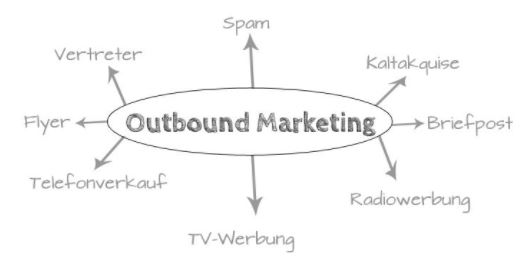
\includegraphics[width=7.5cm]{./Grafiken2/Outbound_Marketing.JPG}
		\caption{Outbound Marketing (/onlinemarketing.de/lexikon/outbound-marketing)}
		\label{Create_Zubereitung}
	\end{minipage}
\end{figure}
Alle diese Methoden haben gemeinsam, dass das Unternehmen sich an den Kunden wendet. Es wird immer eine große Anzahl an Leuten erreicht, jedoch gibt es meist nur wenige die sich überhaupt dafür interessieren, den Beruf ausüben oder Wissen in dem Bereich des Unternehmens haben. Die Strategie hinter diesen Methoden liegt darin, so viele Menschen wie möglich zu erreichen, damit die wenigen welche an dem Produkt interessiert sein könnten ebenfalls die Werbung erhalten. Genauso könnte das Interesse weniger Menschen oder Unternehmen durch diese Methode des Marketings geweckt werden, damit diese das Produkt oder die Dienstleistung des Unternehmens für sich in Anspruch nehmen. 
\newline
Somit gestaltet sich die Neukundenakquise mit Outbound Marketing etwas schwierig, da alle Methoden das Problem haben, zu viele Menschen zu erreichen, die höchstwahrscheinlich nie Kunden werden. Des weiteren kostet es sehr viel Arbeit und Geld, um genug Menschen zu erreichen, damit die richtige Person, die das Produkt oder die Dienstleistung kauft, dabei ist.
\newline 
Eine weitere Methode des Outbound Marketings sind Newsletter oder gezielte Mails an Kunden. Dabei wendet sich das Unternehmen ebenfalls an die Kunden, jedoch in einem viel kleineren Spektrum. Hierbei werden nur Kunden, die auch wirklich an der Dienstleistung oder dem Produkt interessiert sein könnten, diese erhalten. Newsletter müssen abonniert werden und nur wenn ein Account erstellt oder etwas von einer Website gekauft wurde, liegen die entsprechenden Daten vor, damit der Kunde diesen Newsletter erhält. Wurde die Option des Newsletters nicht ausgewählt können und düfren die Kunden diesen nicht erhalten, somit wendet sich das Unternehmen mit dieser Methode meist nur an bereits bestehende oder ehemalige Kunden. 

\subsection{Web Scraping}
Das Web Scraping ist ein Verfahren, welches genutzt wird, um Daten von verschiedenen Websites zu erhalten. Üblicherweise ist es ein automatisierter Prozess, welcher von Computerprogrammen ausgeführt wird. Dabei liest das Programm den Quelltext der gewünschten Website aus und speichert alle erwünschten und gesuchten Daten in einer Datenbank oder Tabelle ab.
\newline
Um dies zu erreichen muss das Programm die URL der Website, die ausgelesen werden soll, kennen. Daraufhin greift das Programm auf den Quelltext zu und liest diesen aus. Sollten Stichwörter auftauchen, die Adressen oder andere personenbezogene Daten suggerieren, werden diese oder die darauf folgenden Zeilen kopiert und in eine Datenbank gespeichert. Telefonnummern, E-Mail Adressen, Adressen und Kontaktdaten haben meist einen speziellen Aufbau, weshalb diese anhand dessen kopiert und gespeichert werden können. E-Mail Adressen beinhalten das '@' Zeichen und Telefonnummern eine Vorwahl. Daran können diese leicht vom Programm identifiziert werden.
\newline
Im Inbound Marketing kann Webscraping genutzt werden, um an die Daten der Kunden zu gelangen, welche erreicht werden sollen oder genügend Interesse gezeigt haben. Web Scraping wird meist zur Neukundenakquise eingesetzt, damit die entsprechenden Kunden diret kontaktiert werden können. Des Weiteren können so Nachforschungen angestellt werden, ob das anzuwerbende Unternehmen überhaupt in das eigene Kundenschema passt. 

\subsection{Data Wrangling}
Unternehmen, die Daten sammeln erhalten diese erst einmal in roher Form. Das bedeutet, dass diese Daten nicht sortiert und geordnet sind. Hierbei hilft das 'Data Wrangling'. Beim 'Data Wrangling' werden die gesammelten Daten genormt. Das Ziel dabei ist Daten,  die aus verschiedensten Quellen kommen, vergleichen zu können. Data Analysten verbringen etwa 70\% - 80\% ihrer Zeit damit die gesammelten Daten zu Normen. Dabei wird geschaut, wie viel Wert die unterschiedlichen Daten für das Unternehmen oder die Analyse hat. Als Nächstes werden die Daten aufgesplittet. Hierbei können aus einer Zeile in der Datenbank gleich mehrere werden. Da manche Daten einfacher zu vergleichen und analysieren sind, wenn sie getrennt werden. 
\newline
'Data Wrangling' ist eine Anstrengende und sehr repetitive Aufgabe. Es wird in 6 unterschiedliche Schritte unterteilt. Der erste Schritt ist die Entdeckung der Daten. Dabei wird herausgefunden, um was für eine Art Daten es sich handelt. Genauso machen sich die Data Analysten in diesem Schritt vertraut mit den Daten.
\newline
Im nächsten Schritt, dem 'Data Structuring', werden die Daten umstrukturiert. Dies muss gemacht werden, da die einzelnen Datensätze meist komplett unterschiedlich sind. Das kann daher kommen, dass die Daten aus unterschiedlichen Quellen stammen oder verschiedene Informationen enthalten. Damit mit den einzelnen Daten gearbeitet werden kann und diese auch miteinander verglichen werden können.
\newline 
Der dritte Schritt nennt sich 'Data Cleaning'. Hier geht es darum Fehler, die beim Importieren aufgetreten sind zu bereinigen oder schlechte Datensätze zu löschen. 
\newline 
Beim 'Data Enriching', dem vierten Schritt, wird sich die Frage gestellt, ob die vorhandenen Daten verschönert oder vermehrt werden müssen.
\newline
Im nächsten Schritt, namens 'Data Validating', kommen Qualitätsprobleme der einzelnen Datensätze zum Vorschein. Dabei wird die Richtigkeit sowie die Authentizität der Datensätze überprüft.
\newline
Das 'Data Publishing' ist der letzte Schritt und hierbei werden die Daten weiter verschoben, damit sie analytisch verarbeitet werden können. 
	
	
	\newpage
	\section{Wie werden Leads generiert ?}
Jedes Unternehmen muss für sich selbst entscheiden, ab wann ein Kunde ein Lead ist oder nur ein Interessent. Manche Firmen sehen einen Interessenten erst als Lead an, wenn ein Formular ausgefüllt und die Personenbezogenen Daten gesammelt wurden. Für andere ist es bereits ein Lead wenn sich aktiv für das Unternehmen interessiert wird. Nachdem dieses Kriterium Unternehmensintern geklärt wurde können Unternehmen beginnen Lead Generierung in ihre Website, Social Media und Werbung zu integrieren. 

\subsection{Website}
Für die Generierung von Leads ist die eigene Website eine der wichtigsten Schwerpunkte, da Unternehmen hier die Freiheit haben alles selbst zu gestalten. Die anzuwendenden Methoden wie Formulare, CTA's, verschiedene Downloads, Landing-Pages und Bewertungen sowie die Selbstdarstellung können frei gewählt werden. Genauso kann entschieden werden wie stark sich auf die einzelnen Methoden konzentriert wird.

\subsubsection{Formulare}
Zu einem Lead gehören Kontaktdaten sowie eine Möglichkeit die Person zu kontaktieren. Die am meisten genutzte Methode, um an diese Daten zu kommen, sind die Formulare. 
\newline 
Ein großer Teil des Inbound Marketings besteht darin dem Interessenten oder der Interessentin immer nur Bruchstücke der gewünschten Informationen zu liefern. Sobald jemand echtes oder großes Interesse zeigt sind Personen bereit diese Daten im Austausch gegen mehr Informationen heraus zu geben. Um an weitere Informationen zu gelangen kann ein Download bereitgestellt oder es muss sich für einen Newsletter angemeldet werden. 
\newline
An diesem Punkt spielen Formulare eine essenzielle Rolle, da so weder ein Kundenkonto erstellt werden muss, noch ist es notwendig, dass sich eine Person bei einer Website registriert. Somit wird es dem potenziellen Lead sehr leicht gemacht Daten anzugeben. Es muss kein aufwendiger Anmeldeprozess durchlaufen werden und die Informationen stehen nach nur drei bis vier Angaben zu eigenen Person bereit. Dabei können die wichtigsten Informationen, wie Name, Vorname, E-Mail Adresse und eventuell auch die aktuelle Stelle im Betrieb abgefragt werden. Formulare können auch mehr abfragen, wobei nicht notwendiger Weise alle Felder Pflichtfelder sein müssen, außer wenn es für das Unternehmen notwendig ist diese Informationen zu erhalten. Zum Beispiel bei einer Hintergrund Überprüfung, wo mehrere Informationen, zur Person, essentiell sind. Jedoch kann es Interessenten abschrecken, wenn sie zu viele Daten über sich heraus geben müssen. Genauso ist es nicht für jedes Unternehmen notwendig so viele Daten über den potenziellen Lead zu erhalten. 
\newline
Ist das Formular ausgefüllt können Kunden gleich auf die gewünschten Informationen zugreifen und das Unternehmen bekommt alle notwendigen Daten, mit welchen der potenzielle Lead erreicht werden kann.

\subsubsection{Bereitstellung von Downloads}
Um Kunden oder potenzielle Leads Neugierig und interessiert an der eigenen Firma zu halten, ist es wichtig nicht alle nötigen Informationen zu sich selbst auf einmal heraus zu geben. 
\newline 
Befindet sich beispielsweise ein Artikel auf der eigenen Website und die Benutzer, welche sich den Artikel durchgelesen haben, möchten mehr Informationen zu dem Thema erhalten, so kann ein Dokument bereitgestellt werden, auf welchem weiter ins Detail gegangen wird. Dabei sollte der Artikel so aufgebaut sein, dass die weitergehenden Informationen beworben werden. Somit bekommt der/die Leser/in einen Einblick in die Materie. Allerdings werden tiefer gehende Informationen vorenthalten, welche erst beim Download des Dokuments oder eines ähnlichen Mediums zur Verfügung stehen.
\newline 
Ist der/die Leser/in interessiert und würde sich gerne weitreichender Informieren, so ist er/sie gezwungen sich die weitergehenden Informationen zu Downloaden. Allerdings sollte an dieser Stelle ein Formular eingebaut werden, welches die Kontaktdaten abfragt. Somit erhalten sowohl die Kunden ihre gewünschten Informationen und können sich anhand dieser bei dem Unternehmen melden, um einen Auftrag abzuschließen. Gleichzeitig hat das Unternehmen nun die benötigten Informationen um den Lead, welcher mit dem ausfüllen den Formulars entstanden ist, weiter zu pflegen, sollte sich dieser nicht für einen Auftrag melden. Sei dies mit persönlich zugeschnittenen E-Mails, basierend auf dem wofür sich der Lead interessiert hat oder welchem bestehenden Kunden der Lead am ähnlichsten ist. Dadurch kann sich das Unternehmen viel spezifischer selbst bewerben. Wenn zu diesem Zeitpunkt die Probleme des Leads feststellbar sind, so kann sich das Unternehmen auch darauf konzentrieren und gleich mit Problemlösungen kommen, um attraktiver für den Lead zu wirken.

\subsubsection{CTA - Call to Action}
Ein CTA, zu deutsch ein Aufruf zum Handeln, ist gut platzierte Werbung die dafür sorgt, dass die einzelnen Besucher der eigenen Website auch auf dieser bleiben. Der Kunde wird aufgefordert weitere Artikel zu lesen oder sich etwas herunterzuladen. Dabei gibt es die verschiedensten Varianten von CTA's. 
\newline
Zum einen gibt es die so genannten Slide-In CTA's, welche wie ein Pop-Up Fenster funktionieren. Sie erscheinen allerdings erst, wenn ein gewisser Punkt auf der Seite erreicht wird. Das kann bedeuten, dass sobald ein Artikel fertig gelesen wurde ein Fenster erscheint, was auf einen weiteren Artikel hinweist, welcher dem Besucher der Website gefallen könnte. Zum anderen kann dies auch eine direkte Anfrage sein, dass sich der Kunde bei der Firma melden soll, wenn Interesse an dem Thema besteht. 
\newline
Für die COM Software GmbH kann dies zum Beispiel bedeuten, dass die Besucher der Homepage, nachdem sie sich eines der Geschäftsfelder durchgelesen haben, aufgefordert werden die Xing Seite des Vertriebsleiters zu besuchen. Dort gibt es weitere Informationen für die Besucher und somit informiert sich die Person immer weiter über das Unternehmen. Ist dies geschehen könnten auf verschiedenste Arten Werbung geschaltet werden, sodass die Person das Unternehmen nicht vergisst und die COM Software für die Planung im nächsten Projekt mit einbezieht. 
\newline 
Das Ziel bei dieser Vorgehensweise ist es immer nur Bruchstücke der Informationen, die der eventuelle Neukunde haben möchte, preiszugeben. Somit informiert sich dieser immer mehr, wenn Interesse besteht und die COM Software kann sich auf diese Person konzentrieren. Dabei kann es sein, dass es für den Kunden von Nöten ist sich für einen Newsletter oder Verteiler anzumelden, um weitere Informationen zu erhalten oder auf diese zugreifen zu können. Ist der Interessent erst einmal im System kann mit Mails oder Nachrichten für die eigene Firma geworben werden. Dabei ist es wichtig eine Kundenbeziehung aufzubauen. Dies kann zum einen dadurch geschehen, dass die Mails aus dem Newsletter oder Verteiler personalisiert sind und von einer echten Person verschickt werden. Dies erzeugt ein Gefühl der Betreuung, da auf die Mails oder Nachrichten geantwortet werden kann. Bei automatisch generierten Mails und Newslettern wissen die Kunden, dass sie in einem Datenverzeichnis mit anderen Unternehmen hinterlegt wurden. Dadurch kommt ihnen die Werbung unpersönlich vor und es kann passieren, dass die Mail oder Nachricht weder gelesen noch geöffnet wird. 

\subsubsection{Landing-Page}
Um Neukunden oder Interessenten Informationen zu liefern und sie als Lead zu gewinnen kann es sehr hilfreich sein eine oder mehrere Landing-Pages in die eigene Homepage zu integrieren. Das Ziel einer Landing-Page besteht darin informativ zu sein. Meist erreicht man diese Seiten nur über Werbung oder Links und kann nicht von der eigentlichen Homepage zu diesen navigieren. 
\newline 
Der Inhalt einer Landing-Page ist sehr spezifisch auf eine Zielgruppe ausgelegt. Dadurch, dass diese Seite nur extern erreichbar ist bekommen auch nur bestimmte Zielpersonen oder Unternehmen einen Zugriff. Der Aufbau und Inhalt einer Landing-Page soll das Interesse dieser einen Zielgruppe wecken, sodass sich die Unternehmen entweder mehr für die ((((eigene Firma)))) interessieren oder gleich kontaktieren, um in die Verkaufsgespräche zu kommen. Dabei werden Informationen zur (((eigenen Firma))) und Dienstleistungen herausgegeben, allerdings nur stückweise, um im Gegenzug für Informationen die Kontaktdaten der jeweiligen Besucher zu erhalten.
\newline 
Somit können mehrere Landing-Pages in die eigene Homepage integriert werden, um die verschiedenen Zielgruppen und Angebote der COM Software GmbH abzudecken. 

\subsubsection{Blog Artikel}
Blog Artikel sind optimale Ort, um CTA's auf der eigenen Website zu platzieren. Hier kann das eigene Produkt beschrieben, eine Problemlösung angeboten oder einfach nur etwas über das eigene Unternehmen erzählt werden. Am besten ist es, wenn auf der gesamten Seite vereinzelt CTA's verteilt werden. Diese sollten zum Inhalt des Blog Artikels passen und auf diesen zugeschnitten sein. Dadurch wird das Interesse des Nutzers aufrecht erhalten, sollte dieser sich weiter für das Thema interessieren. 
\newline 
Blog Artikel sind auf Kunden und Nutzer zugeschnitten, welche sich noch am Anfang des Kaufprozesses befinden, weshalb es für einige Nutzer bedrückend anfühlen kann, sollten sie gleich mit Angeboten überhäuft werden. Teilweise wollen sie sich erst noch weiter in das Thema einlesen oder sich über die verschiedenen Konkurrenten informieren, um die für sie am besten geeignete Lösung zu finden. Aus diesem Grund wird empfohlen, keine Kaufempfehlung in den CTA's auszugeben, sondern weitergehende Informationen anzubieten. Dies kann über eine PDF oder weitere Möglichkeiten geschehen, jedoch sollten die Nutzer ein Formular ausfüllen müssen, um an diese Informationen zu kommen. Alternativ können die CTA's oder auch der Blog Artikel selbst genutzt werden, um den eigenen Newsletter zu bewerben. 
\newline
Durch diese Vielseitigkeit, welche Blogs mit sich bringen, können die unterschiedlichsten Themen beworben werden. Somit kann sich das Unternehmen so breit wie möglich vorstellen, damit die Nutzer eine Idee bekommen, zu was das Unternehmen möglich ist. Allerdings werden viele Blog Artikel benötigt, um sich so breit aufgestellt zu zeigen, da jeder Artikel nur ein Thema behandelt. Darunter sollten sich auch Artikel befinden, welche sich mit Lösungen zu Problemen befassen. Diese dürfen nicht zu sehr ins Detail gehen, da der Kunde nur eine Idee davon bekommen darf, wie ihm das eigene Unternehmen helfen kann. 
\newline
Des Weiteren sollte jeder Blog Artikel ein Produkt oder Dienstleistung bewerben. Dadurch vergisst bleibt der Nutzer auf der eigenen Website und schaut sich die Angebote des eigenen Unternehmens an. 
\newline 
Mit der Hilfe eines Blogs steigt der 'traffic' auf der eigenen Website. Da Nutzer teilweise nur für einen Artikel die eigene Seite besuchen. Allerdings können so sehr viele Leads generiert werden, da einige dieser Nutzer auf der Seite bleiben werden, um sich weitergehend zu informieren. Durch den erhöhten 'traffic' auf der eigenen Website, wird diese bei Suchmaschinen, wie Google oder Bing, höher gelistet. Somit wird sie früher angezeigt und muss nicht extra bei solchen Plattformen beworben werden. 
\newline
Der Aufbau eines Blog Artikels sollte sich auf ein bestimmtes Schlüsselwort beziehen. Somit kann der Artikel leicht über Suchmaschinen oder ähnliches gefunden werden. Außerdem ist von Vorteil, wenn die Artikel nur eine kleine Einsicht in das Thema bieten. Somit kann auf weitere Artikel, Dokumente oder Informationen verwiesen werden, auf welche nur im Austausch gegen Daten, zum Beispiel ein ausgefülltes Formular, zu gegriffen werden kann. 

\subsubsection{Reviews und Selbstpromotion}
Auf der eigenen Website ist es einfach die bekommen Rezensionen und Kritik darzustellen. Des weiteren kann entschieden werden, welche Rezensionen vom Nutzer gesehen werden. Es ist von Vorteil die guten Rezensionen sehr präsent vorzustellen und aufzuzeigen wie Zufrieden die Kunden mit der eigenen Leistung sind. Allerdings sollte darauf geachtet werden nicht zu viel davon zu zeigen, da es schnell manipuliert oder verfälscht wirken kann, wenn nur positives zu finden ist. 
\newline
Um die Zufriedenheit der eigenen Kunden aufzeigen zu können ist eine weitere Möglichkeit deren Logos auf der Website zu präsentieren. Dadurch wird gleichzeitig Vertrauen zum Unternehmen aufgebaut, denn kennen Nutzer diese Firmen oder haben sogar schon Erfahrungen mit ihnen gemacht, so stellen sie direkt eine Verbindung zum eigenen Unternehmen auf. Des weiteren können Kommentare oder eine eigene Sektion für Rezensionen eingebaut werden. Hier können sich die Nutzer belesen und mehr von der Kundenseite des eigenen Unternehmens erfahren. Außerdem können sich Meinungen eingeholt werden und der potenzielle Lead vertieft sein Wissen und eventuell auch Interesse am Unternehmen.
\newline
Um das Vertrauen der potenziellen Leads weiter aufzubauen und um sich selbst zu bewerben können Vertrauenssiegel auf die eigene Website mit eingebaut werden. Dadurch vertrauen Nutzer schneller auf die Echtheit und Integrität eines Unternehmens. Des Weiteren kann auf Blog Artikel oder Seiten der Website verwiesen werden, welche das eigene Unternehmen vorstellen. 


\subsubsection{Search Engine Optimation}
Damit die eigene Website sowie das eigene Unternehmen schnell und einfach entdeckt werden kann ist es wichtig eine gute Internetpräsenz zu zeigen. Dies kann zum einen mit einer ansprechenden Website erreicht werden. Allerdings muss diese Website erst einmal gefunden werden. 
\newline
Hier tragen Suchmaschinen wie 'Google', 'Bing' oder 'DuckDuckGo' eine sehr große Rolle. Je höher eine Website auf der ersten Seite, einer Suchmaschine zu finden ist, desto öfters wird sie besucht. Dabei gibt es die verschiedensten Möglichkeiten, um auf den Suchseiten so weit oben wie möglich zu landen.
\newline
Zunächst sollten die wichtigsten Schlüsselwörter gefunden werden, welche die Nutzer und Kunden verwenden. Mit Hilfe dieser Schlüsselwörter kann die eigene Website in der Rangliste der Suchmaschinen aufsteigen, da sie genau auf die Suchanfragen angepasst wird. Dabei kann der 'Google Keyword Planner' behilflich sein. Dieser gibt Vorschläge von Stichwörtern, welche hilfreich für die eigene Website sein können. 
\newline
Sobald die wichtigsten Schlüsselwörter ausgemacht wurden, müssen diese in die eigene Website integriert werden. Dabei ist es möglich die Überschriften anzupassen, damit diese weiterhin Sinn ergeben und die Schlüsselwörter enthalten. Sind die Überschriften schlüssig, so sind die Nutzer auch mehr gewillt die Seite zu besuchen, weshalb es wichtig ist die Überschriften so aussagekräftig wie möglich zu gestalten. 
\newline
Eine weitere Möglichkeit ist es die Schlüsselwörter in einen Blog Artikel einzubauen oder gleich einen Blog Artikel über die gesamte Thematik zu schreiben. Ein Blog kann generell sehr Hilfreich sein, bei der Search Engine Optimation, da diese regelmäßig geführt werden sollten. Websites die stets neuen Kontent bieten werden ebenfalls stärker gewichtet von Suchmaschinen. Aus diesem Grund ist es wichtig eine gewisse Regelmäßigkeit beim aktualisieren der Website einzuführen. Dabei ist es allerdings nicht notwendig jeden Tag neue Einträge hinzuzufügen, dennoch sollte jeden Monat oder sogar jede Woche die Seite auf den aktuellen Stand gebracht und neue Artikel hinzugefügt werden.
\newline
Es sollte sich auch Gedanken darüber gemacht werden, mit wem konkurriert wird. Es müssen nicht unbedingt Websites sein, die die selbe Dienstleistung oder die selben Produkte anbietet. Es können auch ganz andere Seiten, wie Wikipedia oder Blogs sein. Dabei ist es wichtig zu erörtern, was diese Seiten besser machen und was davon selbst übernommen werden kann.

\subsection{Social Media}



\subsection{Kickback und Follow-Up Emails}
Hat der Kunde seine Daten und Informationen Preis gegeben, so muss der Lead weiter versorgt werden, um ihn als Kunden zu gewinnen. Dabei sind E-Mails sehr hilfreich. Sei es ein Newsletter, personalisierte E-Mails oder eine Danksagung. Wenn sich ein Unternehmen auf diese Weise bei dem Lead meldet wird eine Kundenbeziehung aufgebaut. Die dem Kunden ein Gefühl der Vertrautheit gibt.
\newline
Ist es schon so weit, dass der Lead etwas gekauft oder in Anspruch genommen hat, so ist es wichtig ihn nicht als Kunden zu verlieren. Deshalb sollten Kickback E-Mails versendet werden. Diese können aus einer Danksagung bestehen oder mit neuen Angeboten für weitere Produkte oder Dienstleistungen. Dabei ist es nur wichtig nicht allzu penetrant zu wirken. 
\newline
Allerdings lohnt es sich auch Leads schon bevor sie zu Kunden werden und etwas kaufen mit E-Mails 


\section{RPA - Robotic Process Automation im Inbound Marketing}
Um Leads zu generieren müssen die richtigen Personen angeschrieben werden. Es reicht nicht die eigenen Angebote an die Firmenmail eines Unternehmens zu schicken. Dort gehen die Informationen meist verloren, werden nicht von den richtigen Leuten gesehen oder ignoriert. Um dieses Problem zu umgehen versuchen Marketing Teams sich gleich an die bestimmenden Personen zu wenden, um Ihnen die eigenen Angebote zu präsentieren. Allerdings ist es nicht immer einfach die richtigen Mail Adressen zu haben, insbesondere wenn das Unternehmen noch kein Kunde war. Des weiteren ist dies eine zeitintensive und beschwerliche Aufgabe. 
\newline 
Damit diese Zeit gespart werden kann und sich das Marketing und Vertriebs Team auf wichtigere Themen konzentrieren kann, die das eigene Unternehmen voran bringen, gibt es so genannte RPA's. Diese sind Programme oder Bots, die die Mail Adressen und Kontaktdaten zu Personen finden, welche in das Kunden Schema der jeweiligen Firma passt. Somit kann gleich die richtige Person kontaktiert werden. Sollte diese Person die eigene Firma nicht kennen, so ist es möglich, dass die eigene Firma bei Neukunden präsent gemacht wird. Wenn das Marketing Team mit Hilfe dieser Informationen eine Kundenspezifische Mail verschickt oder anderweitig Kontakt aufnimmt, könnte es sein, dass sich das angesprochene Unternehmen zu der eigenen Firma informiert und sogar als Neukunde gewonnen werden kann. 
\newline 
Hierbei ist es wichtig die bestehenden Kunden gut zu dokumentieren und die Daten ordentlich zu pflegen. Mit Hilfe dieser Daten kann ermittelt werden, ob es sich überhaupt lohnt bei einem Unternehmen anzufragen. 	
	
	
	
	\newpage
	\input{./Abschnitte/Lösungsansätze.tex}
	
	
	\newpage
	\input{./Abschnitte/Empfehlungen.tex}
	
	
	\newpage
	\pagenumbering{Roman}
	\setcounter{page}{5}
	\bibliographystyle{hc-de} %
	
	\addcontentsline{toc}{section}{Literatur} %
	\bibliography{./Literaturverzeichnis} %
	
	%\newpage \section*{}  \thispagestyle{empty} \newpage  \pagestyle{headings}
	%\newpage

\section{Anhang}
%
%\subsection{Sonderformen des Rechnungslegungsprozesses}
%\begin{figure}[H]
%	\centering
%	\includegraphics[width=15cm]{./Grafiken/PDF/rw_Schritt_3a_Rechnungsabwicklung_DZ_VR}
%	\caption{Rechnungsabwicklung DZ BANK AG \& VR Leasing AG}
%	\label{Sonderfall1}
%\end{figure} 
%
%
%\begin{figure}[H]
%	\centering
%	\includegraphics[width=15cm]{./Grafiken/PDF/rw_Schritt_3b_Rechnungsabwicklung_Hays}
%	\caption{Rechnungsabwicklung Hays AG}
%	\label{Sonderfall2}
%\end{figure} 



\end{document}\documentclass[hidelinks,12pt,a4paper]{article}